\documentclass[letterpaper,10pt,serif,draftclsnofoot,onecolumn,compsoc,titlepage]{IEEEtran}

\usepackage{graphicx}                                        
\usepackage{amssymb}                                         
\usepackage{amsmath}                                         
\usepackage{amsthm}                                          
\usepackage{cite}
\usepackage{alltt}                                           
\usepackage{float}
\usepackage{color}
\usepackage[hyphens]{url}
\usepackage{pgfgantt}
\usepackage{rotating}
\usepackage{enumitem}
\usepackage{array}
\usepackage{gensymb}
\usepackage[T1]{fontenc}
\usepackage{balance}
\usepackage[TABBOTCAP, tight]{subfigure}
\usepackage{enumitem}

\usepackage{geometry}
\geometry{margin=.75in}
\usepackage{hyperref}
\usepackage{breakurl}
%\usetikzlibrary{shapes, positioning, calc}
\usepackage{caption}
\usepackage{listings}
%\usepackage[utf8]{inputenc}
%pull in the necessary preamble matter for pygments output

\newcommand{\subparagraph}{}
\usepackage{titlesec}
\usepackage{titletoc}
\setcounter{secnumdepth}{5}
\setcounter{tocdepth}{5}
\titleformat{\paragraph} [hang] {\normalfont\normalsize\bfseries} {\theparagraph} {1em} {}

\usepackage{listings}
\definecolor{dkgreen}{rgb}{0,0.6,0}
\definecolor{gray}{rgb}{0.5,0.5,0.5}
\definecolor{mauve}{rgb}{0.58,0,0.82}

\lstset{
  %frame=tb,
  language=C++, %added
  aboveskip=3mm,
  belowskip=3mm,
  showstringspaces=false,
  columns=flexible,
  basicstyle={\small\ttfamily},
  numbers=none,
  %added
  backgroundcolor=\color{black!5}, % set backgroundcolor
  basicstyle=\footnotesize,% basic font setting
  %added
  breaklines=true,
  breakatwhitespace=true,
  tabsize=4
}

%% The following metadata will show up in the PDF properties
\hypersetup{
   colorlinks = true,
   citecolor = black,
   linkcolor = black,
   urlcolor = black,
   breaklinks = true,
   pdfauthor = {Shu-Ping Chien, Brock Smedley, W Keith Striby Jr},
   pdfkeywords = {CS463 "Senior Project" Final Report},
   pdftitle = {CS463 Final Report},
   pdfsubject = {CS463 Final Report},
   pdfpagemode = UseNone
}

\parindent = 0.0 in
\parskip = 0.1 in
\title{Final Report: Multi-Camera, SoM Based, Real-Time Video Processing for UAS and VR/AR Applications}
\author{Area 51: Shu-Ping Chien, Brock Smedley, W Keith Striby Jr \\ 12 June 2018 \\ CS463, Senior Software Engineering Project, Spring 2018}


\begin{document}
\begin{titlepage}
\maketitle

\begin{abstract}

Write me \\


\thispagestyle{empty}
\end{abstract}
\end{titlepage}

\newpage
\tableofcontents

\newpage

\section{Project Introduction}

\subsection{Problem}
% talk about 1) what's being requested, 2) who requested it & why, & its importance
% 2-3 paragraphs, minimum

\subsection{Persons Involved and Their Role}
% talk about: 1) members of the team, roles, restate client & state his role

\newpage 

\section{Requirements Document}

\documentclass[letterpaper,10pt,serif,draftclsnofoot,onecolumn,compsoc,titlepage]{IEEEtran}

\usepackage{graphicx}                                        
\usepackage{amssymb}                                         
\usepackage{amsmath}                                         
\usepackage{amsthm}                                          
\usepackage{cite}
\usepackage{alltt}                                           
\usepackage{float}
\usepackage{color}
\usepackage{url}
\usepackage{pgfgantt}
\usepackage{rotating}

\usepackage{balance}
\usepackage[TABBOTCAP, tight]{subfigure}
\usepackage{enumitem}

\usepackage{geometry}
\geometry{margin=.75in}
\usepackage{hyperref}
%\usetikzlibrary{shapes, positioning, calc}
\usepackage{caption}
\usepackage{listings}
%\usepackage[utf8]{inputenc}
%pull in the necessary preamble matter for pygments output

%% The following metadata will show up in the PDF properties
\hypersetup{
   colorlinks = true,
   citecolor = black,
   linkcolor = black,
   urlcolor = black,
   pdfauthor = {Shu-Ping Chien, Brock Smedley, and W Keith Striby Jr},
   pdfkeywords = {CS461 "Senior Project" Requirements Document},
   pdftitle = {CS 461 Requirements Document},
   pdfsubject = {CS 461 Requirements Document},
   pdfpagemode = UseNone
}

\parindent = 0.0 in
\parskip = 0.1 in
\title{Requirements Document: Multi-Camera, System-on-Chip (SoC) Based, Real-Time Video Processing for UAS and VR/AR Applications}
\author{Group 51: Shu-Ping Chien, Brock Smedley, and W Keith Stirby Jr \\ 03 November 2017 \\ CS-461, Senior Software Engineering Project, Fall 2017}
\begin{document}
\begin{titlepage}
\maketitle
\begin{abstract}

WRITE ME \\

\end{abstract}
\end{titlepage}
\newpage

\tableofcontents
\newpage

\section{Introduction}

\subsection{Purpose}

This software requirements specification is intended to define the requirements of the 
project of developing a multi-camera, multispectral image processing system, that 
operates on a System-on-Chip (SoC) at near-real-time, for use in ground and air based 
applications. Defined requirements will allow for a contract between us, the 
developers, and Rockwell Collins, our client, on what Rockwell Collins wants us to 
deliver in their desired software. This document is intended for review and reference 
by both the developers and the clients.\\

\subsection{Scope}

The product outlined in this requirements document will be the multi-camera, SoC based,
 real-time video processing for UAS and VR/AR applications. This product will need to 
 be able to generate a stitched video output from a multi-camera input. The product is 
 intended to help initialize our client's development of a cheaper alternative to a 
 product that is already offered to their customers.\\

The software products that will be produced include software for a stitched video output 
from the NVIDIA TX1/2, receiving the input from two visible band cameras. 
The video output is expected to be near real-time, and the latency from the camera 
input to the video output is expected to be improved upon throughout the project. Video 
output stretch goals is to have software that fuses the video output from the input of 
three, four, five, and six cameras, and have up to four infrared band inputs.\\

Output display stretch goals will be to incorporate IMU data, orientation tracking 
data, GPS data, and geolocate imagery. Two final stretch goals are packaging the 
hardware for flight, and interfacing the system to support the client's desired 
cameras for flight use.\\

The goal of the software is to contribute to a project that will assist pilots during 
low visibility conditions during the day, night, and inclement weather for all phases 
of flight. The video input from infrared and visible band cameras combined with 
on-board sensor input, and databases will enhance a pilot's vision for a UAS.\\

\subsection{Definitions, Acronyms, Abbreviations}

\subsubsection{Definitions}

\begin{description}
	\item[geolocate imagery] - 
	\item[low visibility] - 
	\item[multiple cameras] - At least two cameras, but a maximum of six cameras for 
	video input.
	\item[Near real-time] -
	\item[NVIDIA TX1/2] - NVIDIA GPUs, the Jetson TX1 or the Jetson TX2.
	\item[spectral bands] - 
\end{description}

\subsubsection{Acronyms}

\begin{tabular}{|l|l|}
\hline
\textbf{Term} & \textbf{Acronym}\\
\hline
Augmented Reality & AR\\
\hline
Camera Serial Interface & CSI\\
\hline
Enhanced Vision System & EVS\\
\hline
Global Positioning System & GPS\\
\hline
Graphic Processing Unit & GPU\\
\hline
Image Signal Processors & ISP\\
\hline
Inertial Measurement Unit & IMU\\
\hline
Head-up Display & HUD\\
\hline
System-on-chip & SoC\\
\hline
System-on-module & SOM\\
\hline
Size, weight, power and cost & SWaP-C\\
\hline
Three Dimensional & 3D\\
\hline
Two Dimensional & 2D\\
\hline
Video Input & VI\\
\hline
Unmanned Aerial Vehicle & UAV\\
\hline
Unmanned Aircraft System & UAS\\
\hline
Virtual Reality & VR\\
\hline
\end{tabular}

\subsubsection{Abbreviations}

...

\subsection{References}

...

\subsection{Overview}

This project aims to create a device that is capable of combining the video input from 
two or more cameras and produce and output at near real-time. Our proposed solution 
will use an NVIDIA Jetson device, which we will use for its integrated GPU.\\

We need this GPU to combine the images from multiple cameras. The end goal is to have 
a system that uses the input from multiple cameras that operate on the infrared and 
visible light spectral bands. By using these spectral bands, we should be able to 
produce an image that can be used to see in low-visibility situations, such as landing 
a UAV in fog.\\

The images we produce will be 2D representations of our collective image captures. In 
other words, we do not aim to create a 3D image or a dynamic focus image. This is 
certainly possible when using multiple cameras, but we simply aim to use multiple 
cameras on different spectral bands to create one image of one subject that is the 
combination of all images captured by the cameras.\\


\section{Overall Description}

\subsection{Product Perspective}

The system will be self-contained and consists of three parts: one NVIDIA TX1/2, 
one CSI carrier board, and at least two cameras. The cameras connect to the CSI board, 
which is connected to the NVIDIA TX1/2. The NVIDIA TX1/2 is responsible for decoding 
the serial data retrieved by the CSI board from the cameras, and is then be used to 
execute the software for image processing and combining images from multiple cameras.\\

\begin{figure}[H]
	\centering
	\label{fig:CopyOnWriteBefore}
	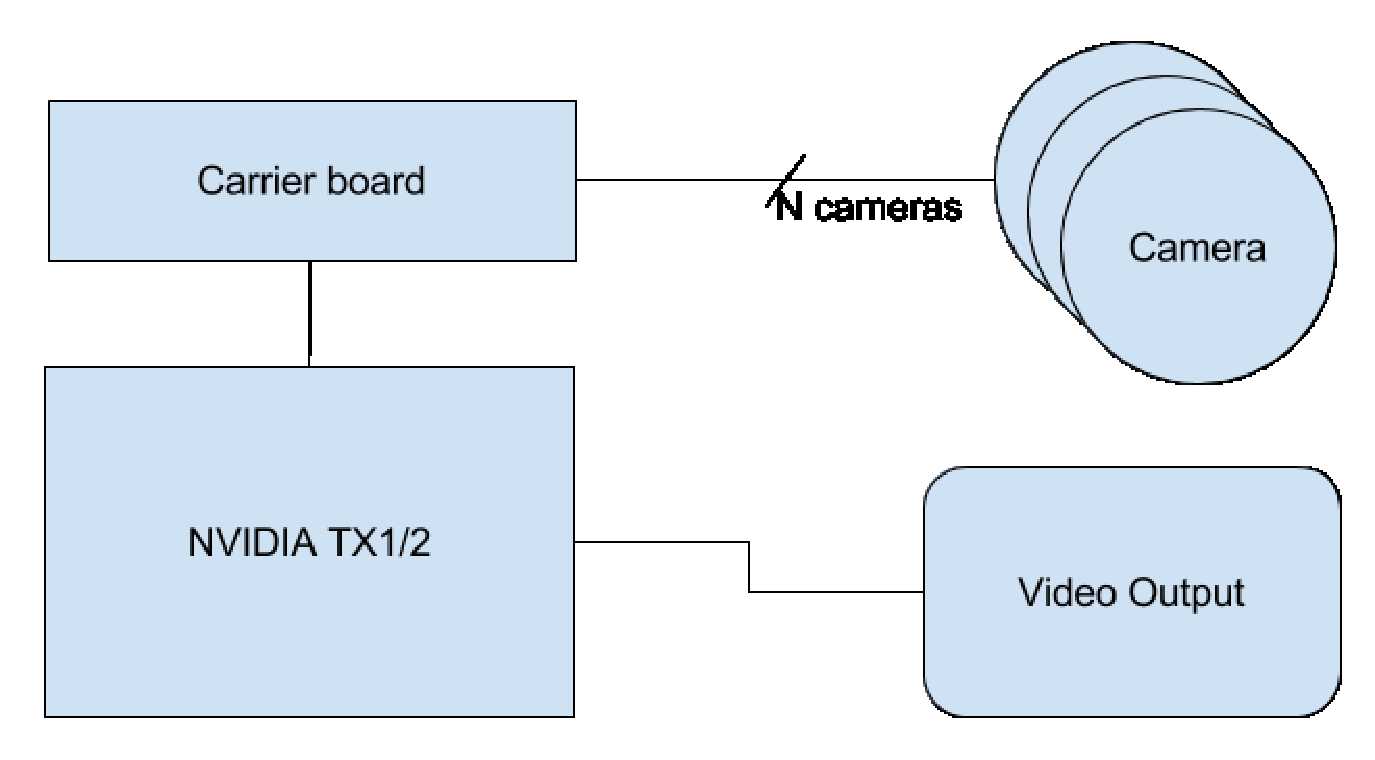
\includegraphics[width=10cm]{images/diagram.eps}
	\caption{Product Block Diagram \label{overflow}}
\end{figure}

\subsection{Product Functions}

The basic functionality of the product will be to produce stitched images on a video 
output that is provided by multiple camera inputs capable of sensing visible and 
infrared spectral bands. These images will be relayed in near real-time so that it 
can be used as a video feed for the pilot of a UAS during low visibility flight 
conditions. \\

A functional stretch goal for video output provided by camera input is to fuse the 
input from the visible and spectral bands, which will overlay the two types of output 
and enhance the vision for a UAS pilot. \\

Output display functional stretch goals will be to provide indications from IMU data, 
orientation tracking data, GPS data, and geolocate imagery and have them displayed 
with the video output provided by the camera input. \\

\subsection{Constraints}

The system must operate in near real-time. In other words, the camera feed(s) must be 
processed quickly enough for the user to make snap decisions based on the feed. The 
NVIDIA board should process each frame before the next one arrives to be processed. 
If we’re recording at 30 frames per second (fps), then each output frame should be 
processed in less than 1/30 of a second.\\

\subsection{Assumptions \& Dependencies}

LIST ITEMS, WRONG, THIS SHOULD BE IN PARAGRAPH FORM\\
Software deployed on NVIDIA TX1/2 with NVIDIA Jetpack from Ubuntu machine
Adequate power supplies being used
Cameras being aimed at same subject; capturing mostly the same image
Each camera works independently of the system

\section{Specific Requirements}
THIS NEEDS TO BE IN PARAGRAPH FORM, WITH SECTIONS FROM THE IEEE STD 830-1998\\
\subsection{Hardware Specifications}
\subsubsection{NVIDIA Jetson TX1/2}
	The NVIDIA TX1/2 will capture images through CSI interface and transfer data into GPU, which is used to combine the images from multiple cameras.\\ 
	The development environment of NVIDIA TX1/2 is available on Ubuntu system, and the module supports softwares for image processing.\\
	The NVIDIA TX1/2 is expected to require adequate power less than 7.5 watts.\\

\subsubsection{CSI Board}
	The carrier board should contain CSI interface, which is used to transfer camera input from up to six cameras to computer.\\
	The CSI board will provide output for a computer with pixel data and signals that can be used for subsequent image processing.\\
	The CSI board should support NVIDIA TX1/2, and the output format of CSI is depending on what cameras we chose.\\

\subsubsection{Cameras}
	The cameras with CSI interface are required in order to transfer image data to computer.\\
	The transfer rate is expected to operate in near-real-time, and the output format from cameras will be accepted by NVIDIA TX1/2.\\
	The cameras should be able to capture images from different spectral channels which includes Infrared, Ultraviolet, and visible light.\\
\subsection{Software Specifications}
	The software is expected to transfer input images into corresponding format for GPU.\\
	The software should be able to fuse images of infrared, ultraviolet, and visible light  and produce 2D video output, and the process should be completed before next input transferred in.\\


\section{Development Schedule}
	\begin{ganttchart}
    	[hgrid, x unit=0.77mm, y unit chart=9.0mm, title label font=\normalsize, time slot format=isodate]
    	{2017-11-01}{2018-05-31}
    	\gantttitlecalendar{year, month=name}\\
    	\ganttbar{Task 1}{2017-11-01}{2017-11-30}\\
    	\ganttbar{Task 2}{2017-11-15}{2018-01-06}\\
    	\ganttbar{Task 3}{2018-01-01}{2018-01-31}\\
    	\ganttbar{Task 4}{2018-01-15}{2018-02-28}\\
    	\ganttbar{Task 5}{2018-03-01}{2018-03-31}\\
    	\ganttbar{Task 6}{2018-04-01}{2018-04-30}\\
    	\ganttbar{Task 7}{2018-05-01}{2018-05-31}\\
	\end{ganttchart}
\begin{center}
	Fig. 2: Project Schedule
\end{center}	

\subsection{Development Schedule Tasks}
Task 1: Have hardware procured and assembled.\\
Task 2: Produce a tiled video output from the input of six cameras.\\
Task 3: Produce stitched video output from the input of two and three cameras, 
and have latency estimates produced.\\
Task 4: Produce a dual stitched video output that is combined into a fused 
five-camera output (stretch goal).\\
Task 5: Incorporate IMU data, orientation tracking data, GPS data, and 
geolocate imagery into the video output (stretch goals).\\
Task 6: Package the system hardware for flight (stretch goal).\\
Task 7: Produce a software interface for the system to accomodate higher 
quality cameras (stretch goal).\\

\end{document}

\newpage

\section{Final Gantt Chart}

make me\\

\newpage

\section{Design Document}

\documentclass[letterpaper,10pt,serif,draftclsnofoot,onecolumn,compsoc,titlepage]{IEEEtran}

\usepackage{graphicx}                                        
\usepackage{amssymb}                                         
\usepackage{amsmath}                                         
\usepackage{amsthm}                                          
\usepackage{cite}
\usepackage{alltt}                                           
\usepackage{float}
\usepackage{color}
\usepackage[hyphens]{url}
\usepackage{pgfgantt}
\usepackage{rotating}
\usepackage{enumitem}
\usepackage{gensymb}
\usepackage[T1]{fontenc}

\usepackage{balance}
\usepackage[TABBOTCAP, tight]{subfigure}
\usepackage{enumitem}

\usepackage{geometry}
\geometry{margin=.75in}
\usepackage{hyperref}
\usepackage{breakurl}
%\usetikzlibrary{shapes, positioning, calc}
\usepackage{caption}
\usepackage{listings}
%\usepackage[utf8]{inputenc}
%pull in the necessary preamble matter for pygments output

%% The following metadata will show up in the PDF properties
\hypersetup{
   colorlinks = true,
   citecolor = black,
   linkcolor = black,
   urlcolor = black,
   breaklinks = true,
   pdfauthor = {Shu-Ping Chien, Brock Smedley, W Keith Striby Jr},
   pdfkeywords = {CS461 "Senior Project" Software Design Description},
   pdftitle = {CS461 Software Design Description},
   pdfsubject = {CS461 Software Design Description},
   pdfpagemode = UseNone
}

\parindent = 0.0 in
\parskip = 0.1 in
\title{Software Design Description: Multi-Camera, SoM Based, Real-Time Video Processing for UAS and VR/AR Applications}
\author{Area 51: Shu-Ping Chien, Brock Smedley, W Keith Stirby Jr \\ 01 December 2017 \\ CS461, Senior Software Engineering Project, Fall 2017}
\begin{document}
\begin{titlepage}
\maketitle
\begin{abstract}

abstract words \\

\thispagestyle{empty}
\end{abstract}
\end{titlepage}

%\newpage
%\tableofcontents

\newpage

\section{Frontispiece}

\subsection{Date of issue and status}

01 December 2017, In-progress \\

\subsection{Issuing Organization}

Rockwell Collins, CS Capstone Group 51, Oregon State University \\

\subsection{Authorship}

Shu-Ping Chien, Brock Smedley, W Keith Stirby Jr \\

\section{Introduction}

\subsection{Purpose}

This document is a general description of design concepts that will be used for our 
multi-camera, SoM based, real-time video processing for UAS and VR/AR applications. 
It is a reference to guide the development of our product.  \\

\subsection{Scope}

Our product will receive input from multiple cameras and then provide a video output at 
near real-time. Our software will receive the pixel data from the cameras and format 
the pixel streams so that image processing can occur. Image processing will then stitch 
the multiple streams of pixels being received to create a combined output. The software 
will be flashed onto the NVIDIA TX1/2, which receives input from the carrier 
board that is connected to the cameras. \\

\subsection{Overview}

The development and design of our product requires: hardware interface and system 
architecture, receiving camera input and formatting for image processing, and image 
processing for video output. The structure of our document reflects these three areas 
of our software required for our product. \\ 

\section{References}

\bibliographystyle{ieeetr}
\bibliography{SDD_Group51}

\section{System Overview}  

\subsection{Identified Stakeholders and Design Concerns}

Rockwell Collins is the primary customer of this product. The company provides 
engineering products in the aviation industry for commercial and military customers. 
Rockwell Collins is the primary user of the product and it is contributing 
to the development of a system that will be used in UAS and VR/AR applications. \\

\subsection{Hardware Context}

The hardware used in our product will be the NVIDIA Jetson TX1/2 as our SoM, 
a carrier board, and cameras. The input from cameras will be transferred through 
carrier boards, and the TX1/2 will format and process the input to produce a 
video output. The software we're developing will be on the TX1/2. \\

\subsection{Software Context}

The software pieces in this project include: GStreamer for transforming video input 
from CSI for image processing, and OpenGL development environment for image processing 
to produce the video output. The pipeline feature in GStreamer will reduce 
cost on time and storage to help achieve near real-time image processing. The OpenGL 
will stitch input images from GStreamer and print the output to the display device. \\

\section{System Architecture}

\subsection{Topic to design}

\subsubsection{subsection topic of topic to design}

words \\

\subsubsection{another subsection topic of topic to design}

words \\

\subsection{Another Topic to design}

\subsubsection{subsection topic of topic to design}

words \\

\subsubsection{another subsection topic of topic to design}

words \\


\nocite{*}
%\newpage
%\bibliographystyle{ieeetr}
%\bibliography{SDD_Group51}
\end{document}

\newpage

\section{Technology Reviews}

\subsection{Shu-Ping's Technology Review}

%\subsubsection{Data storage}
\paragraph{Overview}
NVIDIA Jetson TX1 and TK1 provides 16 GB data storage with eMMC, SDIO, and SATA, and NVIDIA 
Jetson TX2 provides larger storage with 32 GB. In our project, 16 to 32 GB should be enough to 
hold our program because our program receives input video then computes for output will achieve 
near real-time, which means that we do not be able to store many data in our memory. Therefore, 
we will choose suitable data storage and cost SWAP-C. \\


\paragraph{Criteria}
There is not much limitation on data storage since our alternative modules only support eMMC, SDIO, 
and SATA for data storage. Therefore, the chosen data storage requires low size, weight, power, and
 cost (SWAP-C), and we also look for adequate reading speed and stability from a data storage. We 
 will discuss and compare each of these options in the following paragraph. \\

\paragraph{Potential Choices}
\begin{enumerate}
\item{eMMC}
The eMMC is embedded MMC (MultiMediaCard) as an embedded non-volatile memory system, and MMC is a 
memory card standard used for solid-state storage. The embedded card (eMMC) is widely used in the 
industry as a primary means of integrated storage in portable devices because of saved space, and 
almost all mobile phones and tablets used this form of flash for main storage. \\

\item{SDIO}
A SDIO is Secure Digital Input Output card, which is an extension of the SD specification to cover 
Input and Output functions. SDIO cards are functional in host devices designed to support their 
input-output functions, and these devices can support some electronics such as GPS receiver, and 
also interfaces to Wi-Fi, Bluetooth, and Ethernet. The standard size of SDIO is 32.0×24.0×2.1 mm. \\

\item{SATA}
The SATA is Serial AT Attachment, which is a computer bus interface used to connect mass storage 
devices such as hard disk drives and solid-state drives. SATA host adapters and devices communicate 
via a high-speed serial cable over two pairs of conductors, so the efficiency and stability for 
reading and writing data between devices can not be exceed by other data storage. With the advantage
, which is usually used in personal computer or embedded in laptop. \\
\end{enumerate}

\paragraph{Discussion}
Compare the three data storage cards, each technology with different functionalities will be used 
depending different purpose, the SDIO support various input-output functions, and the SATA provides high 
speed for reading and writing data. Since the goal of this project does not require to connect to host 
devices or optimize the speed of reading and writing data, the chosen technology is aimed to cost lower 
SWAP-C. The SDIO and SATA are external cards, so we need extra cost and space if we choose to use them. 
In contrast, because the eMMC is already embedded inside the module, this is the cheapest choice.\\

\paragraph{Conclusion}
We choose to use eMMC because it is already embedded inside every potential SoM in our project, so we do 
not need to have additional space and cost for another data storage. Since our program aims to achieve 
near real-time computation, it will not take much space to store data nor require high reading and 
writing speed with SATA SSD. Therefore, the eMMC is the best choice for data storage in this project that 
the eMMC takes the lowest SWaP-C.\\



\subsubsection{Image processing software}
\paragraph{Overview}
This software intend to transfer input images into a suitable format for image processing in GPU
, which will stitch images from infrared and visible light spectral bands as 2D video output. 
These softwares are usually included in the Jetpack or other development toolkit. In this case, 
the alternative image processing softwares we focus on are available from Jetpack, which are CUDA, 
OpenCV, and OpenGL.\\

\paragraph{Criteria}
Each software would be supported by the chosen module, NVIDIA Jetson TX1/2 or TK1, and where 
the operating system are typically on Ubuntu. In order to fulfil near real-time Latency of 
the data-processing, so the programming will be implemented by the parallel processing. On 
the other hand, considered about the stretch goal, the software will be able to fuse up to 
six camera input.\\

\paragraph{Potential Choices}
\begin{enumerate}
\item{CUDA}
The Jetpack includes CUDA toolkit for Ubuntu, which is a parallel computing platform and 
allows developers to use a GPU for general purpose processing. The CUDA platform is designed 
to work with programming language C and C++. The advantages of CUDA can accelerate download 
and readback to and from the GPU, but there are also some limitations of Interoperability 
with rendering language such as OpenGL.\\

\item{OpenCV}
The Jetpack includes OpenCV library mainly aimed at real-time computer version. OpenCV is 
Open Source Computer Vision Library, which provides basic image processing and video 
processing with build-in algorithm library such as edge detect. Image processing in OpenCV 
can be easier to change images between different color spaces and apply different geometric 
transformations to images.\\

\item{OpenGL}
The Jetpack includes OpenGL 4.3, 4.4 and 4.5 to support GPU developing. OpenGL is Open Graphics Library, 
which is typically used to interact with GPU to achieve accelerated rendering 2D and 3D vector graphics 
with C language. We can handle the image processing with pixel processing path, which the program 
acquires pixels and textures and allow us to operate on those to generate fused images. On the other 
hand, OpenGL also contains the compiler and runtime environment for shaders written in the GLSL shader 
language. The small program of shader runs on the GPU to modify the images depending on the taken input 
from OpenGL textures \cite{shader}.\\ 
\end{enumerate}

\paragraph{Discussion}
In order to achieve the goals of image processing for this project, to fulfil near real-time latency and 
stitch multiple images as one 2D video output, the software we choose should fuse images efficiently. 
Comparing OpenGL with CUDA and OpenCV, the latter softwares provide higher efficiency on reading data and 
computation of image processing. In contrast, the OpenGL shading language enables us to stitch high 
quality images, and the system is more convenient for developer to control more complex conditions since 
we may have multiple input values.\\


\paragraph{Conclusion}
Based on the discussion, we choose to use OpenGL in this project because it is the better choice for 
image processing with multiple video inputs. Since we will have different number and kind of inputs, 
shader language in OpenGL allow us easily to contribute different situations. At the same time, in order 
to accelerate computing vector and pixel information of images, we may include OpenCV library to improve 
the program, or we will write our own algorithm for edge detect. \\


\subsubsection{Media streaming}
\paragraph{Overview}
We need a media streaming software in this project because we have multiple input cameras, and the image 
processing will be implemented with images rather than videos. Therefore, we need a tool to transfer the 
format from input video to image format for image processing and transfer the format back when it is done. 
For instance, we expect the software to read data from the chosen camera, then processes and transfers 
the format and export in the platform for image processing.\\

\paragraph{Criteria}
The chosen media streaming software is also required to be developed on our SoM and the operating 
system. Also, the software should support the format of our video input and be able to connect to 
the image processing software. In the following potential choices, GStreamer and Libargus are 
already included in the Jetpack, so we should be more careful on the limitations when programming 
if we choose to use FFMpeg. \\

\paragraph{Potential Choices}
\begin{enumerate}
\item{GStreamer}
GStreamer is a pipeline-based multimedia framework which links together a wide variety of media processing systems to complete complex workflows. GStreamer is open-source software object and has
 a range of bindings for various languages such as Python and C++. GStreamer processes media
  by connecting a number of processing elements into a pipeline, each element will be grouped and 
  used to different execution \cite{gstreamer}.\\

\item{FFMpeg}
FFmpeg is an open-source multimedia manipulation library of plugins and programs that can be applied to 
various parts of the audio and video processing pipelines \cite{ffmpeg}. FFMpeg includes libav library 
to handle a great quantity of different formats, and the ffmpeg command line program for transcoding 
multimedia files. The FFMpeg supports native NVIDIA GPU hardware accelerated video encoding and decoding 
through the integration of the NVIDIA Video Codec SDK \cite{nvidia}.\\

\item{MEncoder}
MEncoder is a free command line transcoding tool, which can convert and compress general video, audio, 
and image formats, which is usually used with MPlayer as a companion program \cite{mplay}. The same as MPlayer, 
MEncoder is also written in C language, and it features to filter and transform the video and audio 
streams. The filters include cropping, scaling, vertical flipping, etc, the functionality enable user to 
transform and edit their input streams at the same time.\\
\end{enumerate}

\paragraph{Discussion}
Compare the three technologies, FFMpeg supports the most kinds of formats, and GStreamer provides most 
convenient operation to implement streaming at the same time with pipeline system. In contrast, MEncoder 
doesn’t support many formats nor have pipeline interface. Since it is even used with MPlayer, there are 
more limitations to transform data with MEncoder in this project. Then compare FFMpeg with GStreamer, the 
number of supporting formats is not a trouble for GStreamer because the disadvantage can be modified with 
plug-in libraries.\\

\paragraph{Conclusion}
We choose to use GStreamer because the pipeline-based framework lets us easier to control and distribute 
inputs from different cameras. With the arranged input data in order, it allows us to handle processing 
in different conditions if are more than two cameras as input. Moreover, since GStreamer uses a plug-in 
architecture with shared libraries, it is able to support many additional media formats, and which 
includes FFMpeg-based plug-in. Therefore, because of the convenient pipeline-based framework system and 
various media formats, GStreamer is the best choice of media streaming in this project.\\

\newpage

\subsection{Brock Smedley's Technology Review}

%\subsubsection{Development/Deployment Technologies}
The NVIDIA Jetson TX2, the device we plan to implement our solution on, is a System-on-a-Module (SoM) device that hosts an operating system (typically Ubuntu) and allows for several types of development on it. NVIDIA offers a pre-built development environment called Jetpack that includes the operating system and all the software we might need to implement our solution. This is an attractive solution given the simplicity of it, but there are other options. It is also possible to develop our solution on some other workstation and then flash the TX2 system memory with that system's image. We can also install an operating system manually on the TX2 and develop directly on it, as we can with Jetpack, with the caveat that we'll have to manually install all of the software we need. We will examine each of these options in the following paragraphs.

\paragraph{Jetpack}
Jetpack is a software deployment solution that includes an Ubuntu operating system and a bundle of software we might use to develop our solution. Once the TX2 is flashed with the Jetpack image, we can develop directly on the TX2 by connecting peripherals to the device. The software included in Jetpack encompasses a wide variety of disciplines such as machine learning, deep learning, image analysis, system profiling, and more. Also, because the TX2 can connect the internet, we can use the device remotely with SSH.\\

Jetpack is a very attractive option because it is so simple. It includes a majority (if not all) of the software we need to develop our solution, and it flashes the system with Ubuntu which is a very robust and user-friendly operating system. However, if we need more software, we will have to install it ourselves. That is a simple thing to do with Ubuntu, though. Another downfall is that Jetpack takes a long time to install. This is not a problem if we're just installing it once and developing on top of it, but if we want to rebuild the whole system, it will take some extra time.

\paragraph{Remote development}
Another option is to develop the solution on a remote workstation and then flash the TX2 with the newly-developed image for testing. This is the least attractive option because it will require a system memory flash for each build, and memory flashes in general take a considerable amount of time. However, we could take advantage of the extra computing power we can get on a remote workstation (because we can use any workstation) to test computationally-intensive algorithms quickly before deploying them on the TX2 for testing. However, this is still impractical because we can just test algorithms on whatever workstation we want and then access the algorithm's source code (using version control) from the TX2 over the internet and continue testing natively.

\paragraph{Manual OS build}
The last option is to manually install and configure the operating system on the TX2. Using this method, we will have the most control over exactly what our system requirements are and how the system is built. At first glance, this is a slightly less appealing option to Jetpack simply because Jetpack includes so much software that we would otherwise have to install manually. But on the other hand, installing software manually is not very difficult and the process can be scripted. \\

Additionally, the scripts we write to configure the TX2 system environment can be added to version control, which will make our system specifications very transparent and concise. There is also the benefit of saving space; if we install all of our software manually, we can avoid installing programs that we don't need and therefore save space on the TX2. However, space isn't much of a constraint given the TX2's 32GB flash memory capacity. Additionally, Jetpack allows you to individually select the software to install, providing the same memory-saving benefits that manual installation does, without the time-consuming installation process.

\paragraph{Conclusion}
Given consideration to the preceding items, Jetpack appears to be the best software deployment option for this project. Jetpack allows us to easily install the software we need and we can be guaranteed that the image will run on the TX2. Although we won't use scripts to configure the system (which means that it won't be documented in version control), that information can be documented just as well elsewhere, perhaps in a system specification document. Anyone else who wants to recreate our solution can use Jetpack and install the software that we did using it, and can be guaranteed that the system will operate as expected. Additionally, this option will allow for a simplified development process in which we develop directly on the TX2 and manage the system with version control while avoiding unnecessary and time-consuming re-flashing of the system memory.

\newpage
\subsubsection{TX2 System Interfaces}
The NVIDIA TX2 has a variety of system interfaces that can be used to interact with the system during operation. These interfaces will prove useful in later stages of development when we want to test user inputs which will modify parameters of the system while it is in use. The TX2 offers CAN, UART, SPI, I2C, I2S, and GPIOs for serial communication but for brevity, we'll only be looking at I2C, SPI, and GPIO.

\paragraph{I2C}
I2C (Inter-Integrated Circuit) is a serial bus that allows for synchronous communication with the device. With I2C, only two wires are used, one for data and one for the bus clock \cite{i2cBus}. I2C is relatively easy to program for and is very expandable in the sense that it allows interaction with a large number of devices. I2C allows for several different data transmission rates, ranging from 100 kbit/s to 5 Mbit/s. Because of its flexibility and speed, I2C is ideal for interfacing with peripheral devices such as knobs and sensors in real time. \\

I2C is widely used in other applications. Some examples include changing the volume on an intelligent speaker, controlling display brightness in OLED/LCD displays, interfacing with NVRAM chips that store settings, reading configuration data from RAM, and reading real-time clocks. In this regard, I2C is a strong option for interfacing with our system; an application that will require few inputs and outputs and does not require extremely high speed interfacing.

\paragraph{SPI}
SPI (Serial Peripheral Interface bus) is a synchronous serial bus that is commonly used for short-distance communications. Some technologies that utilize SPI include LCD displays and SD cards. SPI has no upper limit on speed and is only limited by the hardware involved. SPI uses four IO lanes (versus I2C's two), but as a result, implementing its use in software is more simplified than I2C. \\

SPI does not support slave acknowledgement, so a master could be transmitting to nothing and not know it. This is less than ideal in a system where intelligent communication between peripherals and the system is required. Additionally, the fact that the bus is meant for short-range communications means that it's not ideal for peripherals that may be relatively distant from the system motherboard.

\paragraph{GPIO}
GPIO (General-purpose input/output) is a serial communications bus that has no specific purpose; its inputs are typically disabled by default \cite{JavaME}. GPIO is particularly effective for interacting with systems that have a limited number of pins, and for reading data from various sensors such as cameras, temperature sensors, and accelerometers. It can also be used to control and write to various devices such as DC motors, audio devices, light-emitting diodes (LEDs), and liquid-crystal (LC) displays. GPIO is generally usable for any peripheral interaction but does not offer especially high speeds or any other feature that might be useful in corner-case-type applications; it's the jack-of-all-trades bus, so to speak. In any case, the use of GPIO can be effective for testing and development, and can typically be replaced with another serial bus like I2C or SPI if necessary since all serial buses have the same fundamental functionality: transmitting data serially.

\paragraph{Conclusion}
Our system will likely use GPIO and I2C for peripheral communication. I2C and GPIO offer robust capabilities and for our application, will do the job well. While we do not know exactly what these ports will be used for yet, it is feasible to assume that we'll need a combination of both speed and data integrity for things such as sensor input and status output. SPI cannot offer data integrity due to its inherent physical short-range limitations. I2C offers high enough speed for the basic sensors and output indicators that we'll eventually use, but it can be overkill for early stages of development. GPIO is very easy to work with physically, and is very commonly used in other microcontrollers, which will make it easy to learn more about during development. At this stage, it is hard to know which one we'll use for which application, so both must be considered during later stages of development.

\newpage
\subsubsection{Operating Systems}
The NVIDIA TX2 allows for a variety of operating systems to be installed. Supported operating systems are built on the Linux 4 kernel. In the following subsubsection, we compare the L4T, ROS, and Ubuntu ARM operating systems, and their potential uses in the project.

\paragraph{L4T (Linux for Tegra)}
L4T is based on Ubuntu, a widely-used operating system that provides a robust repository of software and a user-friendly interface. L4T is the operating system that is provided with NVIDIA Jetpack \cite{jetsonSoft}. Due to the fact that L4T is the default OS installed by Jetpack, the software that NVIDIA recommends for deploying the TX2's operating system, it is a strong contender. In the case of our project, L4T simplifies development in that it is contiguous with the rest of our development platform and it provides a simple and commonly-used environment, which can enable more effective development and future usability.\\

L4T also includes all of the necessary drivers that are needed by the OS to fully take advantage of the TX2. Using another operating system would require manual installation of drivers and software, or a custom image to be flashed onto the system memory. It should also be noted that Ubuntu is NVIDIA's recommended host operating system for deploying the Jetpack image onto the TX2, and therefore we can take advantage of using Ubuntu (L4T is an Ubuntu variant) in both the host and target (TX2) systems to enable more efficient and effective learning during development.

\paragraph{ROS (Robot Operating System)}
ROS is an operating system that was designed to be used in robots. It provides a robust set of tools that allow the OS to interface with other systems easily. ROS is commonly used in robots that have moving parts and whose moving parts are all controlled by one system \cite{introROS}. It allows developers to take advantage of several libraries that simplify the task of controlling multiple components at once. It also offers a declarative programming language known as Robot Description Language that allows the developer to easily model the robot in software for testing and visualization.\\

ROS is a great option for robots that move around or have a lot of moving parts, but our project does not have many moving parts (if any at all). ROS has a lot of interesting functionality that could be useful in other projects, but ours does not need most of the software that ROS includes, and if we do need some of that software, it can be installed manually.

\paragraph{Ubuntu ARM}
The TX2 also supports Ubuntu ARM. Ubuntu ARM is just a version of Ubuntu that runs on the ARM architecture, which is what the TX2 uses in its CPU. The advantage of using Ubuntu ARM is that it has less overhead than L4T because it is a barebones Ubuntu image, meaning that it doesn't come with any pre-installed software that the operating system does not rely on \cite{ARM}. The disadvantage of Ubuntu ARM is that we would have to manually install and configure all of the software that we need or create an image from scratch that has the software and configuration we need.\\ 

One thing that makes the use of Ubuntu ARM attractive is that because the operating system is barebones, although we would have to either make an image from scratch or install everything manually, we could write scripts that do it autonomously and keep them in version control, which would provide a more transparent system description.

\paragraph{Conclusion}
After carefully considering the preceding options, L4T seems to be the best option. Even though it may have more overhead than Ubuntu ARM, space isn't a big concern on the TX2, and it would likely be more effective during development stages given its inherent usability and simplicity. If at some point in the future, system requirements dictated a necessity for better performance, space usage, or efficiency, one could replicate the system configuration of an L4T image on an Ubuntu ARM machine and create a new image from that, but that is something that would be more important for a production system, and those constraints will not be important during the development stage where we will be spending the vast majority of our time.


\newpage

\subsection{Keith Striby's Technology Review}

%\section{Introduction}

The client for our project has requested that we design software for multi-camera video 
streaming, which will be used for UAS (Unmanned Aerial Systems) and VR/AR applications. 
The video output is expected to operate near real-time following image processing, and the multi-camera inputs are 
expected to be stitched and fused on the output display. There are SWaP-C (Size, Weight, Power,
and Cost) constraints and edge computation requirements due to our project's applications. \\

For the duration of the project my role will be to:
\begin{itemize}
	\itemsep-2em
	\item Fulfill the role as liaison between our group and the client. \\
	\item Research and procure hardware required for the product. \\
	\item Assist in software development for stitching and fusing video output. \\
	\item Assist in software development for image processing. \\
\end{itemize}

The remainder of this document investigates three technological areas involved with 
our project. Each section gives a brief description of the technology, explains the 
criteria our choices needed to meet due to the product's application, and displays why 
we would consider each of them. A discussion then follows to compare and contrast each 
technology, and a conclusion then explains why we made our final selection.\\

\section{System-on-Module}

\subsection{Overview}

Selecting our SoM will be the foundation for our project's hardware 
and software choices because of its influence on computational performance, image 
processing, and future product development and expansion. A SoM is capable of offering 
specialized applications a dense computer system in a small package while
maintaining the nature of a microcontroller. SoMs are typically built on a single 
circuit board roughly the size of a credit card, have low power consumption, and 
need to be tethered to a carrier board for input and output peripherals.\\

\subsection{Criteria}

The project requires near real-time image processing to occur in a system that is 
standalone, and conforms to our client's requirements for SWaP-C due to its intended application. For the image processing to 
occur anywhere a UAS travels, the performance of the SoM 
needs to be capable of edge computing while it's up in the clouds.
Multiple camera inputs will be processed through our SoM and their images will be 
stitched, fused, analyzed, and have high-resolution video output. This requires our 
SoM to have a fast, efficient CPU (Central Processing Unit) complex, GPU 
(Graphics Processing Unit)-accelerated computing capable for multimedia streaming, and 
a sizable amount of RAM (Random Access Memory) to aid in computational performance 
and therefore minimize latency.\\

\subsection{Potential Choices}

\subsubsection{NVIDIA Jetson TK1}

The NVIDIA Jetson TK1 is a developer kit built around the Tegra K1 SoC (System 
on Chip (CPU, GPU, ISP (In-system programming) in a single chip)), NVIDIA's first 
mobile processor featuring the same capabilities as a 
modern desktop GPU\cite{JetsonTK1, TK1Wiki}. The Jetson TK1 has the Linux4Tegra (L4T)
OS (operating system) pre-installed, and similar features that you would find on a 
Raspberry Pi and a PC such as GPIO, USB, display interface, SATA, mini-PCIe, and a
fan\cite{RPiHDWR, TK1Wiki}. The Tegra TK1 is built with NVIDIA's Kepler core which 
provides three times the performance than previous NVIDIA GPUs which enables high 
performance computing (HPC) architecture. It also has the NVIDIA CUDA platform to 
create compute-intensive software applications\cite{KeplerArch}. NVIDIA's BSP (board 
support package) and software stack for the Jetson TK1 features Linux Kernel version 
3.10.40 and OpenGL, OpenCL, and CUDA media APIs (Application Program Interfaces)
\cite{TK1L4T}. \\

\subsubsection{NVIDIA Jetson TX1}

The NVIDIA Jetson TX1 is an embedded SoM capable of supporting GPU computing, computer 
vision, graphics, and deep learning making it ideal for embedded AI computing
on an edge device. This SoM has a CPU with four 64-bit A57 ARM cores, and a GPU with 
NVIDIA Maxwell architecture and 256 CUDA cores that provides over 1 TeraFLOPs (floating 
point operations per second) of performance\cite{TX1Wiki, JetsonGenius}. The entire module 
draws just 10W of power making it very energy efficient, and can encode and decode 4K 
video. With 4 GB of RAM and 16 GB of eMMC storage, this module can load software 
applications to on-board storage and process data in RAM\cite{LinuxDot}. The module has 
a 400-pin Samtec board-to-board socket that allows it to connect to NVIDIA's development
board to make use of miscellaneous I/O ports, or to connect to carrier boards that are 
smaller and designed for specific-use applications.\\

NVIDIA provides the Jetson Software Development Pack (JetPack) 3.1, which introduces 
L4T 28.1. Key features in the JetPack 3.1 are TensorRT 2.1, cuDNN 6.0, VisionWorks 1.6, 
CUDA 8.0, Multimedia API, and L4T has Kernel 4.4 for the Jetson TX1. JetPack Developer 
Kit is flashed by the JetPack installer to load the latest OS image, which will install 
developer tools in the host PC and Developer Kit. The host PC is required to have 
Ubuntu Linux x64 (v14.04) to run the JetPack installer\cite{JetPack, JetPackRel}.\\ 

\subsubsection{NVIDIA Jetson TX2}

The NVIDIA Jetson TX2 is the latest SoM by NVIDIA, making it their fastest computing edge
device with 8 GB of RAM and 32 GB of eMMC, twice the memory and storage on the TX1. The 
module has a GPU with NVIDIA Pascal architecture and two NVIDIA Denver2 CPUs plus four 
ARM Cortex-A57 CPUs\cite{TX2Wiki, JetsonFAQ}. The Jetson TX2 can be optimized for 
real-time processing on a UAS, and is 
still power-efficient and small\cite{JetsonGenius}. Additionally, the TX2 has 
Dual Operating Modes, MAX-Q for maximum efficiency and MAX-P for maximum performance, 
where the module can draw 7.5 watts or 15 watts, respectively\cite{TechnoByte}. The TX2 
module has the same 400-pin Samtec board-to-board socket for connection to NVIDIA's 
Developer Kit or carrier board. \\

NVIDIA's JetPack 3.1 is also compatible with the TX2, but features Linux kernel 
4.4\cite{TX2Wiki, JetPackRel}.\\

\subsection{Discussion}

\begin{tabular}{|l|p{5cm}|p{5cm}|p{5cm}|}
	\hline
	\textbf{} & \textbf{Jetson TK1} & \textbf{Jetson TX1} & \textbf{Jetson TX2}\\
	\hline
	\textbf{CPU} & NVIDIA 4-Plus-1 Quad Core ARM Cortex-A15 "r3" @ 2.3 GHz & ARM Cortex-A57 (quad-core) @ 1.73GHz & ARM Cortex-A57 (quad-core) @ 2GHz + NVIDIA Denver2 (dual-core) @ 2GHz\\
	\hline
	\textbf{GPU} & NVIDIA Kepler GK20a with 192 CUDA Cores & 256-core Maxwell @ 998 MHz & 256-core Pascal @ 1300 MHz\\
	\hline
	\textbf{Memory} & 2GB DDR3L 933MHz EMC x16 using 64-bit Width & 4GB 64-bit LPDDR4 @ 1600MHz | 25.6 GB/s & 8GB 128-bit LPDDR4 @ 1866MHz | 59.7 GB/s\\
	\hline
	\textbf{Storage} & 16Gb eMMC 4.51 & 16Gb eMMC 5.1 & 32Gb eMMC 5.1\\
	\hline
	\textbf{Video} & 1080p30 (2x) & 4K x 2K 30 Hz Encode (HEVC), 4K x 2K 60 Hz Decode (10-Bit Support) & 4K x 2K 60 Hz Encode (HEVC), 4K x 2K 60 Hz Decode (12-Bit Support)\\
	\hline
	\textbf{CSI} & 2 fast CSI-2 MIPI camera ports (1x4 + 1x1) & 12 lanes MIPI CSI-2 | 1.5 Gb/s per lane | 1400 megapixels/sec ISP & 12 lanes MIPI CSI-2 | 2.5 Gb/s per lane | 1400 megapixels/sec ISP\\
	\hline
	\textbf{Display} & 1 full-size port & 2x HDMI 2.0 / DP 1.2 / eDP 1.2 | 2x MIPI DSI & 2x HDMI 2.0 / DP 1.2 / eDP 1.2 | 2x MIPI DSI\\
	\hline
	\textbf{Wireless} & 802.11a/b/g/n/ac 2x2 867 Mbps Bluetooth 4.0 & 802.11a/b/g/n/ac 2x2 867 Mbps | Bluetooth 4.0 & 802.11a/b/g/n/ac 2x2 867 Mbps | Bluetooth 4.1\\
	\hline
	\textbf{USB} & USB 3.0 + micro-AB 2.0 & USB 3.0 + 2.0 & USB 3.0 + 2.0\\
	\hline
	\textbf{PCIe} & x1 Lane & Gen 2 | 1x4 + 1X1 & Gen 2 | 1x4 + 1X1 or 2x1 + 1x2\\
	\hline
	\textbf{Other} & UART, I2C, GPIOs & UART, SPI, I2C, I2S, GPIOs & CAN, UART, SPI, I2C, I2S, GPIOs\\
	\hline
	\textbf{Socket} & & 400-pin Samtec board-to-board connector, 50x87mm & 400-pin Samtec board-to-board connector, 50x87mm\\
	\hline
	\textbf{Thermals} & & -25\degree C to 80\degree C & -25\degree C to 80\degree C\\
	\hline
	\textbf{Power} & 15W & 10W & 7.5W\\
	\hline
	\textbf{Dimensions} & 5" x 5" board & 1.96" x 3.42" module & 1.96" x 3.42" module\\
	\hline
	\textbf{Weight} & 120 grams & 88 grams & 85 grams\\
	\hline
	\textbf{Cost} & \$192 each (Developer Kit) & \$299 at 1K units (module) & \$399 at 1K units (module)\\
	\hline
\end{tabular}
\newline
\newline
\newline
Note: Operating Lifetime is 5 years for Jetson Commercial Products.\\
Table References: \cite{TK1Wiki, TK1Power, TK1Rev, JetsonFAQ, TegraK1, TK12Comp, JetsonGenius, TX1PS, TX2DS}\\

NVIDIA's Jetson TK1 Development Kit (dev kit) was used in comparison to the Jetson TX1 
and Jetson TX2 modules because the NVIDIA Tegra K1 processor is not available on a 
module. The size of the Jetson TK1 dev kit puts it at a 
disadvantage when comparing it to the size, weight, and max power draw of the Jetson 
TX1 and TX2 modules. The major disadvantage that the TK1 has in comparison to the TX1 
and TX2 is the amount of CSI cameras it can accommodate. \\

NVIDIA was capable of doubling or enhancing all active processing components on the 
TX2 in comparison to the TX1, and both modules have the same dimensions. With NVIDIA's 
latest release of Jetpack 3.1 being compatible for both TX1 and TX2 both modules 
have near-equal software support, where most differences are application 
versions\cite{TX1Wiki, TX2Wiki, JetPackRel}. \\  

\subsection{Conclusion}

The final selection for our product's SoM is between the Jetson TX1 and TX2, and will 
be dependent on the software development and carrier board testing. Both the 
Jetson TX1 and TX2 offer great SWaP-C requirements for our product's application and 
are compatible with the carrier boards that have been selected to test. Additionally, 
both the Jetson TX1 and TX2 are capable of supporting up to six cameras through their 
12 CSI(Cameral Serial Interface)-2 lanes. \\

\section{Carrier Board}

\subsection{Overview}

Carrier boards (also known as baseboards) are designed with application-specific 
interfaces and peripherals, and offer scalability and flexibility due to the target 
application only being supported. A carrier board is always used in tandem with a SoM, 
and by separating the two a SoM can be upgraded without the possible redesign of the 
carrier board\cite{ToradexSBC, ArrowCB, ToradexCBQ}.\\

\subsection{Criteria}

The application of our product requires a carrier board that is capable of interfacing 
with multiple high-resolution cameras to produce a quality video output. The NVIDIA Jetson TX1 
and TX2 allow camera input through: USB 2.0 and 3.0 ports, MIPI CSI-2 camera ports, and 
potentially through the mini-PCIe ports\cite{JetsonCams}. MIPI CSI-2 cameras are roughly a few millimeters 
in size and allow for quick image processing due to the images being processed directly 
through the SoM's ISP. The MIPI CSI-2 camera interface is capable of supporting 1080p, 
4k, 8k video and it's the most widely used camera interface for mobile 
applications\cite{MIPIOverview}. With that, our carrier board must be capable of interfacing  
six CSI-2 camera inputs simultaneously. \\

\subsection{Potential Choices}

\subsubsection{Auvidea J106 Carrier Board}

The Auvidea J106 carrier board plugs into the 400-pin Samtec board-to-board connector 
on the Jetson TX1 and TX2, and is the same shape and size as both modules. 
It supports up to six MIPI CSI-2 15 pin camera input connections to our 
desired NVIDIA Jetpack SoM and also has an IMU (inertial measurement Unit). Additional 
interfaces featured on the J106 are: microSD, USB 
3.0, Micro USB, UART, 1 Gb Ethernet, I2C, SATA, 4x PCIe, CAN, and a mini 
HDMI\cite{AuvideaJ106}. The J106 board costs \$240 each at 1K units\cite{AuvideaQuote}.\\

The Auvidea M100 and M110 motherboards connects to the J106 board and all are the same 
size. Both motherboards are port extenders for the J106, which can allow the use of 
additional peripherals for input processing in the Jetson TX1 or 
TX2\cite{AuvideaMBoards}. \\

\subsubsection{Colorado Engineering, Inc X-Carrier Board}

The X-Carrier Board designed and by Colorado Engineering, Inc (CEI) is capable of 
supporting six 15 pin MIPI CSI-2 cameras through the Auvidea J20-2 camera adapter. The 
J20-2 board plugs into the bottom of the X-Carrier, and the Jetson TX1 or TX2 plugs 
into the 400-pin Samtec board-to-board connector on top. A Jetson TX1 or TX2 board does 
mount to the X-Carrier board but the X-Carrier is slightly larger. The X-Carrier has a built-in IMU 
and the following interfaces: HDMI 2.0, MicroSD, SATA 2.0, USB 2.0, USB 3.0, 1 Gb 
Ethernet, x1 and x4 PCIe Gen 2, 2x UART, 2x SPI, 3x I2C, 3x I2S, and GPIOs. CEI is  
developing various I/O modules to connect to the X-Carrier and include: radar, comms, 
active IR, passive IR, CANBus, and others\cite{CEIXpdf, J20TechRef, AuvideaJ20}. The X-Carrier costs \$285 each 
and the J20-2 costs \$129 each, both at 1K units\cite{SpacelyQuote, AuvideaQuote}. \\
	
\subsubsection{Connect Tech, Inc Spacely Carrier}

The Spacely Carrier designed by Connect Tech, Inc has six built-in MIPI CSI-2 camera 
inputs with 30 pins and offers a built-in expansion for a GPS/GNSS module. The NVIDAIA 
Jetson TX1 or TX2 module plugs into the 400-pin Samtec board-to-board connector on top 
of the Spacely Carrier. The following interfaces are on the Spacely Carrier: HDMI, 2x 
Gigabit Ethernet, 2x Micro USB 3.0, 2x USB 2.0, 1x USB OTG, 1x USB 2.0 to Mini-PCIe 
Slot, 1x mSATA, 2x 3.3V from Jetson UART0 and UART1, 1x Mini-PCIe, 1x microSD, 1x CAN 2.b 
Port, 1x I2C Link, 1x SPI Channel, and 14x GPIO\cite{SpacelyUG}. The Spacely Carrier 
costs \$411 each at 1K units.\\

\subsection{Discussion}

\begin{tabular}{|l|p{5cm}|p{5cm}|p{5cm}|}
	\hline
	\textbf{} & \textbf{J106 Carrier} & \textbf{X-Carrier} & \textbf{Spacely Carrier}\\
	\hline
	\textbf{CSI} & 6 2-lane CSI-2 (15 pin) & 6 2-lane CSI & 6 x2 Lane MIPI CSI-2 or 3 x4 Lane MIPI CSI-2 (30 pin)\\
	\hline
	\textbf{USB} & 2x USB 3.0, 1x Micro USB & 1x USB 3.0, 1x Mini-USB 2.0 & 2x Micro USB 3.0, 2x USB 2.0, 1x USB OTG, 1x USB 2.0 to Mini-PCIe Slot \\
	\hline
	\textbf{SATA} & 1x SATA & 1x SATA 2.0 & 1x mSATA Full Size \\
	\hline
	\textbf{Display} & 1x mini HDMI & 1x HDMI 2.0 & 1x HDMI \\
	\hline
	\textbf{PCIe} & 4x PCIe & x1 and x4 PCIe Gen 2 & 1x Mini-PCIe \\
	\hline
	\textbf{Other} & UART, Gb Ethernet, I2C, 1x CAN & MicroSD, 1 Gb Ethernet, 2x UART, 2x SPI, 3x I2C, 3x I2S, and GPIOs & 2x 3.3V from Jetson UART0 and UART1, 1x MicroSD, 1x CAN 2.b Port, 1x I2C Link, 1x SPI Channel, and 14x GPIO \\
	\hline
	\textbf{Thermals} &  & -20\degree C to 55\degree C & -40\degree C to 85\degree C \\
	\hline
	\textbf{Voltage} & 12V (4 pin), range: 7V to 17V & 12V to 19V & 12V to 22V \\
	\hline
	\textbf{Dimensions} & 1.96" x 3.42" board & 3.43" x 2.8" board & 4.92" x 3.74" board \\
	\hline
	\textbf{Weight} & 2.6 grams & 6.5 grams & 90.7 grams \\
	\hline
	\textbf{Cost} & \$240 each at 1K units & \$285 each at 1K units & \$411 each at 1K units \\
	\hline
\end{tabular}	
\newline
\newline
\newline
Note: The Auvidea M100 and M110 motherboards are \$129 each at 1K units, and the 
J20-2 board is \$129 each at 1K units. \\
Table References: \cite{AuvideaJ106, MouserJ106, CEIX, CEIXpdf, SpacelyUG, SpacelyQuote, CEIQuote, AuvideaQuote}\\

The J106 carrier board size is form fitting with the Jetson TX1 or TX2 modules and 
maintains this size when even used with the Auvidea M100 or M110 motherboards, unlike 
the X-Carrier's and Spacely Carrier's larger board dimensions. However, the J106 carrier board 
offers limited interfaces in comparison to the X-Carrier and Spacely Carrier boards due 
to its size and relies on its 4x PCIe slots for future options like a GPS/GNSS module. The 
X-Carrier does rely on the Auvidea J20-2 board to connect to for supporting  
camera input whereas the J106 and Spacely Carrier have all six MIPI CSI-2 ports directly 
installed. The major benefit to the Spacely Carrier's size is that it has a large 
amount of USB ports and miscellaneous I/O ports and a built-in expansion for a 
GPS/GNSS module. Although, the J106 and X-Carrier Boards have built-in IMUs whereas the 
Spacely Carrier does not.\\

\subsection{Conclusion}

The final selection for our product's carrier board is dependent on multiple variables, 
all of which will be determined during software development and testing. All three of 
the companies 
designed and developed their carrier boards for specific use with the Jetson TX1 and 
TX2 modules. Each carrier board offers subtle and unique 
advantages over the other, and it's difficult to say which one will be capable of 
providing the best solution without adequate testing. \\

\section{Camera Case}

\subsection{Overview}

The Raspberry Pi (v2) cameras selected for developing our software have an exposed circuit 
board and camera lens. These cameras should be enclosed for protection and mounted to 
provide consistent testing of the software being produced. Camera mounting and positioning
will need to remain in the same known setup while developing software for multiple camera 
input. \\

\subsection{Criteria}

The case needs to be capable of performing two basic functions for the camera, which 
are protecting the camera and holding the camera securely. The case should be specifically 
designed for our Raspberry Pi cameras to ensure these two basic functions are easily 
met. For mounting of the case to another object it will be beneficial for it to 
have screw holes on it. \\

\subsection{Potential Choices}

\subsubsection{Adjustable Pi Camera Mount}

This camera mount made by Pimoroni is as basic as they come and are \$5 each. The mount 
consists of a two-piece bracket, one to mount the camera to and another to fix the 
mount. However, the support bracket and camera bracket snap together. This camera 
mount includes screws and hex-nuts to secure the camera to the bracket\cite{AdjCamMt}. \\

\subsubsection{Raspberry Pi Camera Case/Enclosure}

SB Components created a camera case specifically designed for the Raspberry Pi camera 
and snaps together to firmly hold the camera in place. The case has two screw holes for 
mounting, comes with screws and tape, and are \$6 each\cite{BlueCase}. \\

\subsubsection{Adafruit Raspberry Pi Camera Board Case}

This Adafruit Raspberry Pi enclosure is sleek, snaps closed, and has four pegs inside making a 
secure hold on the camera. To mount the case are two slots and a 
one-quarter inch tripod mount nut. A hole on the lid of the case to prevents 
distorting camera images. Our Raspberry Pi Camera v2 is slightly thicker than the 
original camera that the case was designed for, and it is recommended to remove a spacer from 
the circuit board to prevent blurry images. These cases are priced at \$3 each\cite{adafruitCase}.\\

\subsection{Discussion}

Each option provides a different stance on simplicity, caters to custom mounting 
options, and is specifically designed for Raspberry Pi. The adjustable mount 
by Pimoroni offers no protection unlike SB Components and Adafruit's cases. The 
mounting holes on SB Components enclosure does come with screws for them but with 
just a little extra effort the Adafruit case can be just as secure. Adafruit's 
case has a sleek and minimalist design and may be more versatile for mounting, but 
the big blocky SB Components case positions the camera vertically and has the 
screw holes on its horizontal surface. \\

\subsection{Conclusion}

The SB Components camera case was chosen because its enclosure can hold the camera's 
field of view vertical while the mounting holes are on the horizontal axis. Pimoroni's
mount was ruled out since the two camera cases have the best mounting options for 
securing the cameras in place. The Adafruit's case will require 
more effort and creativity to mount the cameras securely for testing stitched or 
fused camera inputs, and is why SB Components case is slightly more appealing.\\

\newpage

\section{Weekly Blog Posts}


\newpage

\section{Final Poster}


\newpage

\section{Project Documentation}


\newpage

\section{Recommended Technical Resources for Learning More}


\newpage

\section{Conclusions and Reflections}


\newpage

\section{Appendix 1: Essential Code Listings}
% doesn't have to be everything, but there should be stuff here for someone to learn from


\nocite{*}
\newpage
\bibliographystyle{ieeetr}
\bibliography{PFPR_Group51}
\end{document}
